%CLASSE DOCUMENTO - LINGUA E DIMENSIONE FONT
\documentclass[corpo=11pt,numerazioneromana]{toptesi}

%%%%%%%%%%%%%%%%%%%%%%%%%%%%%%%%%%%%%%%%%%%%%%%%%%%%%%%%%%%%%%%

% INCLUSIONE PACCHETTI
\usepackage[classica]{topfront}
\usepackage[utf8]{inputenc} %utf8
\usepackage[italian]{babel}
\usepackage[T1]{fontenc}
\usepackage{blindtext}
\usepackage{graphicx,wrapfig}
\usepackage{booktabs}
\usepackage{lmodern}
\usepackage{varioref}
\usepackage{url}
\usepackage{array}
\usepackage{paralist}{\obeyspaces\global\let =\space}
\usepackage{verbatim}
\usepackage{subfig}
\usepackage{tabularx}
\usepackage[table,xcdraw]{xcolor}
\usepackage{amsmath}
\usepackage{amsfonts}
\usepackage{float}
\usepackage{amssymb}
\usepackage{multicol}
\usepackage{multirow}
\usepackage{listings}
\usepackage[pass]{geometry}
\usepackage[figuresright]{rotating}
\usepackage{algorithm}
\usepackage{setspace}
\usepackage{algorithmic}
\usepackage{amsmath}
\usepackage[babel]{csquotes}
\usepackage{hyperref}
\usepackage[toc, acronym]{glossaries}
\usepackage[backend=biber,bibencoding=ascii]{biblatex}


\renewcommand*{\glstextformat}[1]{\textcolor{blue}{#1}}


%%%%%%%%%%%%%%%%%%%%%%%%%%%%%%%%%%%%%%%%%%%%%%%%%%%%%%%%%%%%%%%

% CONFIGURAZIONE LINK E RIFERIMENTI
\hypersetup{%
    pdfpagemode={UseOutlines},
    bookmarksopen,
    pdfstartview={FitH},
    colorlinks,
    linkcolor={black}, %COLORE DEI RIFERIMENTI AL TESTO
    citecolor={blue}, %COLORE DEI RIFERIMENTI ALLE CITAZIONI
    urlcolor={blue} %COLORI DEGLI URL
}
\newcommand{\MYhref}[3][blue]{\href{#2}{\color{#1}{#3}}}%

%%%%%%%%%%%%%%%%%%%%%%%%%%%%%%%%%%%%%%%%%%%%%%%%%%%%%%%%%%%%%%%

% CONFIGURAZIONE LISTATI/CODICE - CANCELLARE SE NON NECESSARIO
% PYTHON - BIANCO E NERO
\lstset{%
	captionpos=b,
	language=Python,
	basicstyle =\small\ttfamily,
	keywordstyle=\color{black}\bfseries,
	breaklines=true,
	breakatwhitespace=true,
	frame=lines,
	numbers=left,
	numberstyle=\footnotesize,
}

%%%%%%%%%%%%%%%%%%%%%%%%%%%%%%%%%%%%%%%%%%%%%%%%%%%%%%%%%%%%%%%

% FRENCHSPACING VA _SEMPRE_ ABILITATO PER DOCUMENTI IN ITALIANO
\frenchspacing

%%%%%%%%%%%%%%%%%%%%%%%%%%%%%%%%%%%%%%%%%%%%%%%%%%%%%%%%%%%%%%%

%DEFINIZIONE SEZIONI IN NUMERAZIONE ROMANA
%ELENCO DEI LISTATI/CODICI
\makeatletter
\newcommand\listofcodes{%
 \iffrontmatter\else\frontmattertrue\fi
 \if@openright\cleardoublepage\else\clearpage\fi
 % change the meaning of \chapter in a group
 \begingroup\def\chapter##1{\@schapter}
 \phantomsection % for the hyperlink
 \addcontentsline{toc}{chapter}{Elenco dei listati}
 \lstlistoflistings
 \endgroup
} 
\makeatother

\addto\captionsitalian{%
  \renewcommand{\lstlistlistingname}{Elenco dei listati}%
  \renewcommand{\lstlistingname}{Listato}%
}

%%%%%%%%%%%%%%%%%%%%%%%%%%%%%%%%%%%%%%%%%%%%%%%%%%%%%%%%%%%%%%%

% INFORMAZIONI PDF - PERSONALIZZARE
\pdfinfo{%
  /Title    (Sviluppo di una Web Application per l’ottimizzazione del processo di onboarding flussi)
  /Author   (Oleg Stoianov)
  /Subject  ()
  /Keywords ()
}
%%%%%%%%%%%%%%%%%%%%%%%%%%%%%%%%%%%%%%%%%%%%%%%%%%%%%%%%%%%%%%%
% Glossario

\makeglossaries
\label{glossario}

\newglossaryentry{front-end}
{
    name=front-end,
    description={la parte visibile all'utente di un programma e con cui egli può interagire, tipicamente un'interfaccia utente}
}
\newglossaryentry{back-end}
{
    name=back-end,
    description={programma e architettura con il quale l'utente interagisce indirettamente, di solito attraverso l'utilizzo di un'applicazione front-end}
}
\newglossaryentry{FULL-STACK}
{
    name=FULL-STACK,
    description={identifica lo sviluppo di un intero sistema informatico o applicazione dal front-end al back-end e al codice software che li collega}
}

\newglossaryentry{bestpractices}
{
    name=best practices,
    description={ Modo di fare che garantisce i migliori risultati in specifiche e note circostanze}
}

\newglossaryentry{ict}{
    name=ICT,
    description={“Information and Communication Technologies”, ICT è l’insieme delle tecnologie che forniscono l’accesso alle informazioni attraverso le telecomunicazioni. A differenza dell’Information Technology, l’ICT è più focalizzata sulle tecnologie di comunicazione, come internet, reti wireless, telefoni cellulari e altri mezzi di comunicazione}
}

\newglossaryentry{applicazioneweb}
{
    name=Web Application,
    description={identifica un’applicazione  risiedente  in  un  Server  Web  alla  quale  si  accede  tramite  un  browser  Internet  o  un  altro  programma  con  funzioni  di  navigazione  operante secondo gli standard del World Wide Web}
}

\newglossaryentry{agile}
{
    name=Agile,
    description={Lo sviluppo agile consiste nel rilasciare rapidamente modifiche al software in piccole porzioni con l'obiettivo di migliorare la soddisfazione dei clienti. Con l'adozione dello sviluppo agile i vari team costituiti da pochi sviluppatori ciascuno collaborano direttamente con i rappresentanti aziendali tramite incontri periodici durante l'intero ciclo di vita dello sviluppo del software}
}


\newglossaryentry{systemintegrator}{
    name=System Integrator,
    description={Nel campo dell'IT gli integratori di sistemi connettono sistemi eterogenei in modo che questi possano comunicare, processare, salvare, categorizzare dati}
}

\newglossaryentry{B2B}{
    name=B2B,
    description={"business-to-business", descrive le transazioni commerciali che intercorrono tra imprese industriali, commerciali o di servizi all'interno dei cosiddetti mercati interorganizzativi}
}

\newglossaryentry{EDI}{
    name=EDI,
    description={"Electronic Data Interchange", è l'interscambio di dati tra sistemi informativi, attraverso un canale dedicato e in un formato definito in modo da non richiedere intervento umano salvo in casi eccezionali}
}

\newglossaryentry{WWW}{
    name=WWW,
    description={"World Wide Web", è uno dei principali servizi di Internet, che permette di navigare e usufruire di un insieme molto vasto di contenuti amatoriali e professionali (multimediali e non) collegati tra loro attraverso legami (link), e di ulteriori servizi accessibili a tutti o ad una parte selezionata degli utenti di Internet}
}

\newglossaryentry{framework}
{
    name=framework,
    description={astrazione che fornisce un insieme di classi, strumenti, utilità con funzionalità generiche, adattabili al domino applicativo specifico per l’utilizzo desiderato.
    Un framework fornisce una maniera standard di produrre applicazioni che seguono principi consolidati e ne facilita l’integrazione}
}

\newglossaryentry{businesspartner}{
    name=business partner,
    description={Soggetto che va ad affiancarsi ad un'impresa in un rapporto di collaborazione continuata, in merito alla distribuzione, promozione e vendita dei suoi prodotti}
}

\newglossaryentry{MFT}{
    name=MFT,
    description={"Managed File Transfer", Il trasferimento di file gestito si riferisce a un software o un servizio che gestisce il trasferimento sicuro di dati da un computer a un altro attraverso una rete (ad esempio Internet). Il software MFT è commercializzato per le aziende come alternativa all'utilizzo di soluzioni di trasferimento di file ad hoc, come FTP, HTTP e altri}
}

\newglossaryentry{BPML}{
    name=BPML,
    description={"Business Process Modeling Language", è un linguaggio basato su XML per la modellazione dei Business Process. Fornisce un modello di esecuzione astratto per processi aziendali collaborativi e transazionali basato sul concetto di una macchina a stati finiti transazionale}
}

\newglossaryentry{ip}{
    name=indirizzo IP,
    description={è un numero del datagramma IP che identifica univocamente un dispositivo detto host collegato a una rete informatica che utilizza l'Internet Protocol come protocollo di rete per l'instradamento/indirizzamento}
}

\newglossaryentry{tcpip}{
    name=TCP/IP,
    description={indica una famiglia di protocolli di rete legati da dipendenze d'uso su cui si basa il funzionamento logico della rete Internet, rappresenta lo standard  \textit{de facto} nell'ambito delle reti dati}
}

\newglossaryentry{charset}{
    name=charset,
    description={è l'associazione fra un insieme di codici numerici e i rispettivi caratteri di un determinato linguaggio}
}
\newglossaryentry{codiceabi}{
    name=codice ABI,
    description={"Associazione Bancaria Italiana", è un numero composto da cinque cifre e rappresenta l'istituto di credito. Ogni banca possiede un codice ABI che viene assegnato proprio dall'Associazione bancaria italiana}
}

\newglossaryentry{diagrammagantt}{
    name=diagramma di Gantt,
    description={usato principalmente nelle attività di project management, è costruito partendo da un asse orizzontale a rappresentazione dell'arco temporale totale del progetto e da un asse verticale a rappresentazione delle mansioni o attività che costituiscono il progetto}
}

\newglossaryentry{designpattern}{
    name=design pattern,
    description={è un concetto che può essere definito "una soluzione progettuale generale ad un problema ricorrente". Si tratta di una descrizione o modello logico da applicare per la risoluzione di un problema}
}

\newglossaryentry{API}{
    name=API,
    description={"Application Programming Interface", sono un set di definizioni e protocolli con i quali vengono realizzati e integrati software applicativi. Consentono la comunicazione tra prodotti o servizi con altri prodotti o servizi senza sapere come vengono implementati}
}

\newglossaryentry{DBMS}{
    name=DBMS,
    description={"Database Management System", è un sistema software progettato per consentire la creazione, la manipolazione e l'interrogazione efficiente di database}
}

\newglossaryentry{schema}{
    name=schema,
    description={In un dizionario di dati, uno schema di database indica come le entità che compongono il database si relazionano tra loro, comprese le tabelle, le viste, le procedure memorizzate e altro ancora}
}


\newglossaryentry{log}{
    name=log,
    description={file costituito da un elenco cronologico delle attività svolte da un sistema operativo, da un database o da altri programmi, generato per permettere una successiva verifica}
}

\newglossaryentry{UML}{
    name=UML,
    description={è un linguaggio che permette, tramite l’utilizzo di modelli visuali, di analizzare, descrivere, specificare e documentare un sistema software anche complesso}
}

\newglossaryentry{IDE}{
    name=IDE,
    description={"Integrated Development Environment", è un software che, in fase di programmazione, supporta i programmatori nello sviluppo del codice sorgente di un programma}
}

\newglossaryentry{repository}{
    name=repository,
    description={è un archivio in grado di contenere dati e relativi metadati. Può offrire un sistema di
versionamento in grado di tenere traccia delle modifiche effettuate al suo interno}
}

\newglossaryentry{debugging}{
    name=debugging,
    description={indica l'attività che consiste nell'individuazione e correzione da parte del programmatore di uno o più errori (bug) rilevati nel software}
}

\newglossaryentry{DAO}{
    name=DAO,
    description={"Data Access Object", è un pattern architetturale per la gestione della persistenza: si tratta fondamentalmente di una classe con relativi metodi che rappresenta un'entità tabellare di un DBMS relazionale}
}

\newglossaryentry{sistemidistribuiti}{
    name=sistemi distribuiti,
    description={è una porzione di software che assicura che un insieme di calcolatori appaiano come un unico sistema coerente agli utenti del sistema stesso}
}

\newglossaryentry{URL}{
    name=URL,
    description={"Uniform Resource Locator",  è una sequenza di caratteri che identifica univocamente l'indirizzo di una risorsa su una rete di computer, come ad esempio un documento, un'immagine, un video, tipicamente presente su un host server e resa accessibile a un client}
}

\newglossaryentry{HTTP}{
    name=HTTP,
    description={"HyperText Transfer Protocol", è un protocollo a livello applicativo usato come principale sistema per la trasmissione d'informazioni sul web}
}

\newglossaryentry{REST}{
    name=REST,
    description={"Representational State Transfer", rappresenta un sistema di trasmissione di dati su HTTP.Il principio fondamentale è l'esistenza di risorse (fonti di informazioni), a cui si può accedere tramite un identificatore globale}
}

\newglossaryentry{opensource}{
    name=open source,
    description={un software è reso tale per mezzo di una licenza attraverso cui i detentori dei diritti favoriscono la modifica, lo studio, l'utilizzo e la redistribuzione del codice sorgente. Caratteristica principale dunque delle licenze open source è la pubblicazione del codice sorgente}
}






 









%%%%%%%%%%%%%%%%%%%%%%%%%%%%%%%%%%%%%%%%%%%%%%%%%%%%%%%%%%%%%%%

% LISTA DEI CAPITOLI DA INCLUDERE - PERSONALIZZARE
\includeonly{%
chap_introduzione,%
chap_azienda,%
chap_stage,%
chap_strumenti,%
chap_analisi,%
chap_progettazione,%
chap_verifica,%
chap_conclusioni,%
app_a,%
}

%%%%%%%%%%%%%%%%%%%%%%%%%%%%%%%%%%%%%%%%%%%%%%%%%%%%%%%%%%%%%%%

% FILE DI BIBLIOGRAFIA
\addbibresource{bibliography.bib}

%%%%%%%%%%%%%%%%%%%%%%%%%%%%%%%%%%%%%%%%%%%%%%%%%%%%%%%%%%%%%%%

% INIZIO DOCUMENTO
\begin{document}

%%%%%%%%%%%%%%%%%%%%%%%%%%%%%%%%%%%%%%%%%%%%%%%%%%%%%%%%%%%%%%%

% FRONTESPIZIO - PERSONALIZZARE
% ELIMINATE LE VOCI CHE NON VI SERVONO

% UNIVERSITA - NOME
%\ateneo{Università degli Studi di Milano Bicocca}

% FACOLTA - DICITURA - CANCELLARE O DECOMMENTARE
%\FacoltaDi{Faculty of}
% FACOLTA - NOME
%\facolta{Scuola di Scienze
%Dipartimento di Informatica, Sistemistica e Comunicazione
%}

% CORSO DI LAUREA - DICITURA (MANTENERE LO SPAZIO) - CANCELLARE O DECOMMENTARE
%\CorsoDiLaureaIn{Master of Science in }
% CORSO DI LAUREA - NOME
%\corsodilaurea{Corso di laurea in Informatica}

% TIPOLOGIA TESI
%\TesiDiLaurea{Tesi di Laurea Triennale}

% TITOLO
%\titolo{Sviluppo di una Web Application per l’ottimizzazione onboarding flussi}


% RELATORE/I - DICITURA - CANCELLARE SE UN SOLO RELATORE
%\AdvisorName{Relatori}
% RELATORE - PROF. NOME E COGNOME
%\relatore{prof.\ Guido Giuseppe Fiorino}


% CANDIDATO - DICITURA (MANTENERE I DUE PUNTI) - CANCELLARE O DECOMMENTARE
%\CandidateName{Candidate:}

% CANDIDATO - NOME E COGNOME
%\candidato{Oleg Stoianov}
% CANDIDATA - ELIMINARE O SOSTITUIRE CON IL PRECEDENTE
%\candidata{Tinasa de Tinasis} 
% SECONDO CANDIDATO - ELIMINARE O DECOMMENTARE
%secondocandidato{Bombo de Bombis}
%secondacandidata{Bomba de Bombis}

% LOGO UNIVERSITA
%\logosede{images/logo_unimib}

% DATA - MESE ANNO
%\sedutadilaurea{Luglio 2020}

%\frontespizio

\begin{titlepage}
        
        \noindent
        \begin{minipage}[t]{0.18\textwidth}
            \vspace{-4mm}{
\includegraphics[scale=1.15]{images/logo_unimib.pdf}}
        \end{minipage}
        \begin{minipage}[t]{0.83\textwidth}
        {
                \setstretch{1.42}
                {\textsc{Università degli Studi di Milano - Bicocca}} \\
                \textbf{Scuola di Scienze} \\
                \textbf{Dipartimento di Informatica, Sistemistica e Comunicazione} \\
                \textbf{Corso di laurea in Informatica} \\
                \par
        }
        \end{minipage}
        
	\vspace{40mm}
        
	\begin{center}
            {\LARGE{
                    \setstretch{1.2}
                    \textbf{Sviluppo di una Web Application per l’ottimizzazione del processo di onboarding flussi}
                    \par
            }}
        \end{center}
        
        \vspace{40mm}

        \noindent
        {\large \textbf{Relatore:} Prof. Guido Giuseppe Fiorino } \\

        %\noindent
        %{\large \textbf{Correlatore:} Dott. CCC DDD}
        
        \vspace{10mm}

        \begin{flushright}
            {\large \textbf{Relazione della prova finale di:}} \\
            \large{Oleg Stoianov} \\
            \large{Matricola 829519} 
        \end{flushright}
        
        \vspace{25mm}
        \begin{center}
            {\large{\bf Anno Accademico 2019-2020}}
        \end{center}

        \restoregeometry
        
\end{titlepage}



%%%%%%%%%%%%%%%%%%%%%%%%%%%%%%%%%%%%%%%%%%%%%%%%%%%%%%%%%%%%%%%

%INTERLINEA - DEFAULT 1 - NON ESAGERATE, NON SUPERATE MAI 1.3 ;)
%\interlinea{1.2}

%%%%%%%%%%%%%%%%%%%%%%%%%%%%%%%%%%%%%%%%%%%%%%%%%%%%%%%%%%%%%%%

\frontmatter

% DEDICA - PERSONALIZZARE
% VSPACE - PROPORZIONE USATA PER CENTRATURA VERTICALE DEL TESTO
% FLUSHRIGHT - ALLINEAMENTO ORIZZONTALE A DESTRA
%\vspace*{\stretch{1}}
%\begin{flushright}
%\noindent

%\end{flushright}
%\vspace*{\stretch{6}}
%\cleardoublepage


% CITAZIONE - PERSONALIZZARE
% VSPACE - PROPORZIONE USATA PER CENTRATURA VERTICALE DEL TESTO
% FLUSHRIGHT - ALLINEAMENTO ORIZZONTALE A DESTRA
%\vspace*{\stretch{1}}
%\begin{flushright}
%\noindent
%Citatemi dicendo che sono stato citato male.

%\textit{Groucho Marx}
%\end{flushright}
%\vspace*{\stretch{6}}
%\cleardoublepage

%%%%%%%%%%%%%%%%%%%%%%%%%%%%%%%%%%%%%%%%%%%%%%%%%%%%%%%%%%%%%%%

% RINGRAZIAMENTI - PERSONALIZZARE
\ringraziamenti
Un ringraziamento speciale alla mia famiglia, in particolare a mia madre e mio padre: è grazie a loro sostegno e al loro incoraggiamento se oggi sono riuscito a raggiungere questo traguardo.

Ringrazio la mia fidanzata Veronica per avermi trasmesso la sua forza e il suo coraggio. Grazie per tutto il tempo che mi hai dedicato. Grazie per la pazienza che hai avuto con me. Grazie perché ci sei sempre stata. 


Ringrazio i miei colleghi, nonchè amici, con cui ho condiviso l’intero percorso universitario. Grazie ai quali ho superato i momenti più difficili, e ho vissuto a pieno l'esperienza universitaria.


Infine, dedico questa tesi a me stesso, ai miei sacrifici e alla mia tenacia che mi hanno permesso di arrivare fin qui.




%%%%%%%%%%%%%%%%%%%%%%%%%%%%%%%%%%%%%%%%%%%%%%%%%%%%%%%%%%%%%%%

% ABSTRACT - PERSONALIZZARE
% \sommario
% \hypertarget{sommario}{}
% \label{chap:sommario}
% Il seguente documento descrive il lavoro svolto dal laureando Oleg Stoianov durante il periodo di stage presso L’azienda Innovery S.p.a.
% L’obiettivo dell’attività era quello di sviluppare una \gls{applicazioneweb} per ottimizzare il processo di onboarding di flussi logici e delle relative informazioni degli attori coinvolti durante lo scambio dei dati all’interno di un \gls{systemintegrator}, utilizzato presso l’azienda SIA S.p.A, per processi \gls{B2B} ed \gls{EDI}.


%%%%%%%%%%%%%%%%%%%%%%%%%%%%%%%%%%%%%%%%%%%%%%%%%%%%%%%%%%%%%%%

% INDICI - ELIMINARE GLI INDICI NON NECESSARI

% INDICE GENERALE
\tableofcontents

% INDICE DELLE FIGURE
\listoffigures

% INDICE DELLE TABELLE
\listoftables

% % INDICE DEI CODICI
% \listofcodes

%%%%%%%%%%%%%%%%%%%%%%%%%%%%%%%%%%%%%%%%%%%%%%%%%%%%%%%%%%%%%%%

\mainmatter

% INCLUSIONE FILE CAPITOLI - PERSONALIZZARE - TENERE COERENTE CON LISTA IN ALTO
\chapter{Introduzione}
\label{chap:introduzione}

\section{Scopo del documento}
\label{sec:scopodeldocumento}
Questo documento è la relazione finale su quanto svolto durante il periodo di stage come conclusione del percorso di laurea triennale.   \\

Esso è strutturato in maniera tale da:
\begin{itemize}
    \item Dare un idea del contesto lavorativo in cui è stato svolto lo stage
    \item Definire le richieste del committente del progetto
    \item Riportare la pianificazione del lavoro
    \item Riportare l'analisi effettuata
    \item Spiegare la soluzione proposta
    \item Descrivere le tecnologie e gli strumenti utilizzati
    \item Riportare il risultato e le conclusioni
\end{itemize}


Il tutto utilizzando conoscenze pregresse, formazione specifica aziendale ed un affiancamento ad un Team di sviluppo.





%This is a reference to a chapter \ref{chap:quo}. This is a reference to a figure \ref{fig:doge}. This is a reference to some code \ref{lst:hello}. This is a citation \cite{famous:paper}.

%\lstinputlisting[label=lst:hello, firstline=2, lastline=4, caption={I directly included a portion of a file}]{code/hello.py}

%\begin{lstlisting}[language=Java, label=lst:java, caption={Some code in another language than the default one}]
%public void prepare(AClass foo) {
%        AnotherClass bar = new AnotherClass(foo)
%}
%\end{lstlisting}

% DA RIMUOVERE - LOREM IPSUM PER DIMOSTRAZIONE
%\foreignlanguage{english}{\Blindtext}

%\begin{figure}
%\begin{center}
%\includegraphics[width=0.5\columnwidth]{images/doge.png}
%\end{center}
%\caption{This is not a figure. It's a caption.}
%\label{fig:doge}
%\end{figure}

%\section{}
\chapter{Le aziende}
\label{chap:aziende}
\section{Innovery S.p.A.}
\label{sec:innovery}

\begin{figure}
\begin{center}

\includegraphics[width=0.5\columnwidth]{images/logo_innovery.png}
\end{center}
\caption{Logo Innovery S.p.A.}
\label{fig:logo_innovery}
\end{figure}

\subsection{Profilo aziendale}
\label{subsec:innoprofilo}


Innovery è una società multinazionale nata nel 2001, che opera nell’area dei servizi ICT per le medie e grandi Aziende. Negli anni ha esteso il suo portfolio a tutte le aree della sicurezza informatica, coprendone tutti gli aspetti. Questo ha permesso di ampliare il suo mercato spingendosi sui territori internazionali. Ad oggi, infatti conta 10 sedi in tutto il mondo, coprendo oltre il territorio italiano, anche quello spagnolo e latinoamericano. Innovery offre soluzioni e servizi personalizzati, per soddisfare le esigenze specifiche dei clienti, completi di progettazione, realizzazione e supporto.\cite{innovery}


\subsection{Servizi offerti}
\label{subsec:innoservizi}
I servizi sono articolati in 10 unità operative: Security, Managed Services, Big Data, Mobile Solutions, E-Business, Billing  System, High  Performance  Computing, Physical  Security, Health Care, Funded  Projects. \cite{innoveryservizi} \\


Tra i più rilevanti abbiamo : \begin{itemize}
    \item Security Privacy Governance \\ 
La Security Privacy Governance rappresenta lo sguardo più generale sulla sicurezza e la
privacy; è essenziale per una Privacy by Design \& by Default e per ottenere la conformità
alle norme sulla sicurezza e sulla privacy (GDPR).
    
    \item Identity \& Access Management \\ 
L’Identity \& Access Management (IAM) è il punto di partenza essenziale di ogni sistema
di gestione della sicurezza delle informazioni: si tratta di disporre di soluzioni integrate
che consentano l’identificazione di individui e componenti dei sistemi, e di stabilire
quando e quali azioni possano svolgere sulle diverse risorse aziendali.

    \item Ethical Hacking/Forensic Analysis \\
L’attività di Vulnerability Assessment e Penetration Testing (VA/PT) consente di
avere una piena consapevolezza dello stato dell’infrastruttura e di tracciare un’efficace
Remediation Roadmap delle vulnerabilità identificate

    \item Network Security \\
La messa in sicurezza delle reti è la prima tappa della roadmap verso un’infrastruttura tecnologica sicura. Per la sicurezza dei dati e delle infrastrutture offre servizi specialistici basati sulle migliori tecnologie: Firewall; Intrusion Detection \& Prevention System (IDS/IPS); End Point Protection System; Advanced Persistent Threat (APT) Defense System.

    \item B2B Integration \& Managed File Transfer \\
L’integrazione End-to-End e l’efficienza del flusso di transazioni fra i sistemi interni e la
propria “comunità di business” è garantito da robusti strumenti come l’IBM Sterling B2B Integrator and Managed File Transfer Solutions (Sterling MFT). Sulla base di tale piattaforma
tecnologica, Innovery offre soluzioni come l’Innovery User Gateway (IUG), una
console Web di gestione centralizzata delle funzionalità della piattaforma Sterling Integrator;
\end{itemize}

\clearpage

\section{SIA S.p.A.}
\label{sec:sia}

\begin{figure}
\begin{center}

\includegraphics[width=0.5\columnwidth]{images/logo_sia.png}
\end{center}
\caption{Logo SIA S.p.A.}
\label{fig:logo_sia}
\end{figure}

\subsection{Profilo aziendale}
\label{subsec:siaprofilo}
SIA - società controllata da CDP Equity - è leader europeo nella progettazione, realizzazione e gestione di infrastrutture e servizi tecnologici dedicati alle Istituzioni Finanziarie, Banche Centrali, Imprese e Pubbliche Amministrazioni, nei segmenti Card \& Merchant Solutions, Digital Payment Solutions e Capital Market \& Network Solutions. Il Gruppo SIA eroga servizi in oltre 50 paesi e opera anche attraverso controllate in Austria, Croazia, Germania, Grecia, Repubblica Ceca, Romania, Serbia, Slovacchia, Sudafrica e Ungheria. La società ha inoltre filiali in Belgio e Olanda e uffici di rappresentanza in Inghilterra e Polonia.\cite{sia}


\subsection{Servizi offerti}
\label{subsec:siaservizi}

Tra i servizi offerti: processing delle carte di credito e debito, pagamenti elettronici, servizi di rete, piattaforme per i mercati finanziari.\cite{siasoluzioni} \\

In particolar modo: 

\begin{itemize}
    \item Card Management \\
    Soluzione innovativa e sicura di card management per singoli istituti di credito, grandi gruppi bancari, processor di carte e aziende. SIA supporta gli issuer nell’emissione di tutti i tipi di carte.
    
    \item Sistemi di pagamento tra cui:
    \begin{itemize}
        \item Servizi di tesoreria 
        \item Processing
        \item Accesso al Clearing
        \item Settlement
        \item Grandi Basi Dati
    \end{itemize}
    
    \item Servizi di rete \\
    SIAnet Financial Ring, si tratta di un'infrastruttura di connettività multisede a 10 Gbps sicura, affidabile e a bassa latenza, accessibile tramite 9 PoP (Point of Presence) a Milano, Londra, New York, Budapest e Francoforte che offrono una soluzione di connettività diretta e dedicata ai principali CSD, broker e sedi di negoziazione, consentendo in tal modo di ridurre i costi legati alla complessità.
    
    
    \item Blockchain \\
    Gestione digitalizzata delle fideiussioni basata su tecnologia blockchain.
    
    \item Sicurezza fisica \\
    SIA intelliFENCE è il brand con cui Emmecom firma le sue soluzioni per l’antintrusione, la videosorveglianza e il safety: una suite modulare e integrata, basata sui protocolli di comunicazione standard del settore bancario e offerta nella logica più vicina alle esigenze del cliente.
\end{itemize}



















\chapter{Stage}
\label{chap:stage}


\section{Introduzione al progetto}
\label{sec:introstage}
Lo stage ha avuto una durata di 3 mesi, dal 07/10/2019 al 07/01/2020 presso la sede milanese di SIA S.p.A in Via Privata Francesco Gonin 36. \\

Come accennato nell' \hyperlink{introduzione}{introduzione}, il contenuto dello stage verte principalmente sullo sviluppo di una \textit{Web Application}, commissionata dall'azienda SIA S.p.A all'azienda Innovery S.p.A.
Il progetto in questione ha come obiettivo principale l'ottimizzazione del processo di \textit{onboarding} di flussi logici che devono essere condivisi tra Business Partners e che devono passare attraverso un \gls{systemintegrator}, \textit{IBM® Sterling B2B Integrator}. \\

\subsection{IBM® Sterling B2B Integrator}
IBM® Sterling B2B Integrator è un motore di transazione che esegue \textit{Business Process}, supporta lo scambio di messaggi elettronici ad alto volume, l'instradamento complesso, la traduzione, il trasferimento gestito di file (\gls{MFT}) e l'integrazione flessibile con più sistemi interni e partner commerciali esterni. Include strumenti di gestione visiva per la configurazione e la visibilità dei flussi di lavoro, le attività del sistema e dei partner commerciali, le mappe di traduzione e l'implementazione dei \textit{Business Process}. Funziona con centinaia di protocolli aziendali e standard di comunicazione emergenti \cite{ibmsterling}.

Tra i componenti principali di questo complesso sistema abbiamo:
\begin{itemize}
    \item \textit{Business Process}: un flusso di attività ordinato e orientato al raggiungimento degli obiettivi aziendali. Ogni \textit{Business Process} è definito da un unico documento \gls{BPML}.
    \item \textit{Services}: una risorsa che è possibile configurare per svolgere un'attività. 
    \item \textit{Adapters}: casi speciali di \textit{Services} che interagiscono con sistemi esterni o che archiviano o gestiscono dati di stato al di fuori del contesto del flusso di lavoro.
\end{itemize}



\clearpage

\begin{figure}
\begin{center}
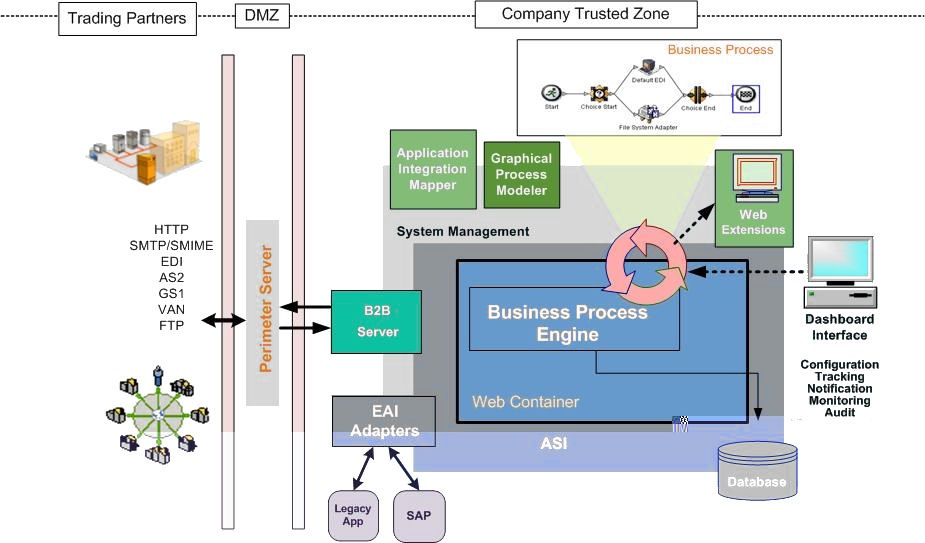
\includegraphics[width=1.0\columnwidth]{images/ibmarchitecture.jpg}
\end{center}
\caption{Architettura software IBM® Sterling B2B Integrator}
\label{fig:archi_sterling}
\end{figure}


\subsection{Architettura già esistente}
L'azienda SIA S.p.a presenta un'infrastruttura di tipo \textit{cluster}, un insieme di computer connessi tra loro tramite una rete telematica. Scopo del \textit{cluster} è distribuire un'elaborazione molto complessa tra i vari computer, aumentando la potenza di calcolo del sistema e garantendo una maggiore disponibilità di servizio, a prezzo di un maggior costo e complessità di gestione dell'infrastruttura \cite{cluster}. Come si evince dalla figura \ref{fig:archi_sia} sono presenti due macchine sulle quali è installato IBM® Sterling B2B Integrator, ambedue i nodi condividono lo stesso database e inoltre si scambiano informazioni riguardanti il carico, lo stato dell'applicazione e del nodo. L'architettura presenta inoltre i seguenti componenti per aumentare la sicurezza dell'infrastruttura:
\begin{itemize}
    \item \textit{Firewall}: hardware e software per controllare il traffico in ingresso/uscita di una rete fidata rispetto a reti non sicure
    \item \textit{Application Proxy}: interfaccia di comunicazione in una rete per monitorare il traffico fra applicazioni
    \item \textit{DMZ}: zona demilitarizzata, indica una rete di computer, che funge tra due reti da zona cuscinetto con un proprio indirizzo IP e le delimita mediante regole di accesso rigide
\end{itemize}
Per mantenere l'integrità dell'architettura, la \textit{Web Application} verrà installata su entrambi i nodi dove è installato il prodotto IBM® Sterling B2B Integrator, sarà però attivata solo su uno dei due. (In \ref{fig:archi_sia} IBM® Sterling B2B Integrator è abbreviato con SFG)



\clearpage

\begin{figure}
\begin{center}
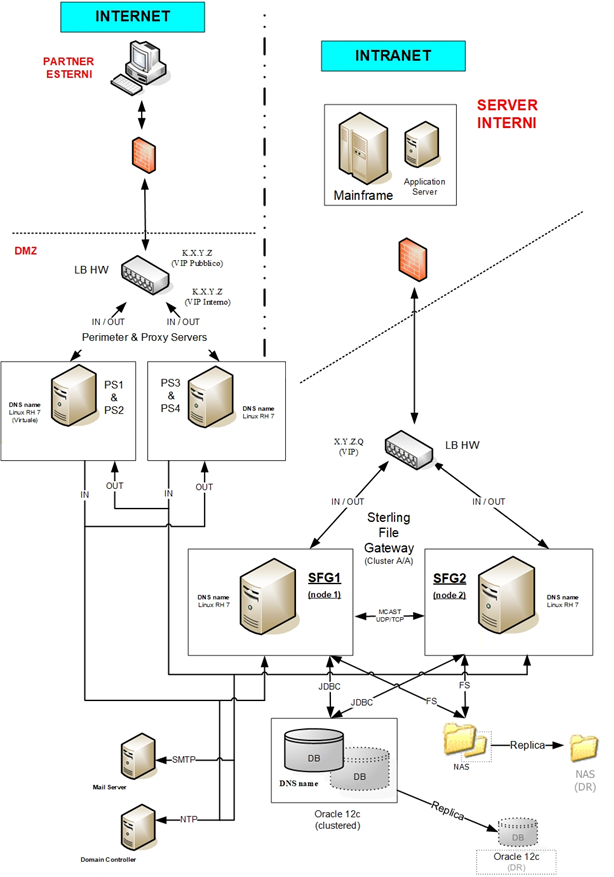
\includegraphics[width=0.9\columnwidth]{images/siaarch.png}
\end{center}
\caption{Architettura installata in SIA S.p.A}
\label{fig:archi_sia}
\end{figure}

\clearpage


\subsection{Processo di onboarding flussi}
\label{subsec:onboarding}
Per processo di \textit{onboarding} di flussi logici, si intende la registrazione di informazioni utili per la gestione e l'implementazione di regole di instradamento per i file che passano attraverso il prodotto IBM® Sterling B2B Integrator.
Le informazioni necessarie possono essere suddivise in 3 categorie: informazioni sistemistiche, operazionali e metadati.

Per informazioni sistemistiche intendiamo tutte quelle informazioni riguardanti:
\begin{itemize}
    \item \Gls{ip}
    \item Porta \gls{tcpip}
    \item Protocollo utilizzato
\end{itemize}
Queste informazioni servono per poter definire \textit{"come"} un \gls{businesspartner} ha intenzione di interfacciarsi con il \gls{systemintegrator}, con lo scopo di inviare e/o ricevere file. \\
Le informazioni operazionali rappresentano informazioni riguardanti alle operazioni che possono essere effettuate sul file prima di essere consegnato al \gls{businesspartner} destinatario. Tra le operazioni possibili abbiamo:
\begin{itemize}
    \item Ridenominazione: rinomina il nome del file.
    \item Backup: salva una copia del file.
    \item Compressione: effettua una riduzione delle dimensioni del file attraverso uno specifico algoritmo. 
    \item Decompressione: riporta un file precedentemente compresso alle condizioni iniziali.
    \item Cifratura: applica un algoritmo di cifratura specifico per rendere il contenuto del file incomprensibile.
    \item Decifrazione: applica un algoritmo di cifratura specifico per rendere il contenuto del file leggibile.
    \item Codifica \gls{charset}: converte i caratteri del \gls{charset} iniziale in caratteri di un altro \gls{charset}.
\end{itemize}

Per poter instradare correttamente un file i metadati necessari sono:  \gls{businesspartner} mittente, destinatario e regola che identifica univocamente il file. La regola richiesta è nella nomenclatura del file da gestire, quest'ultima dovrà avere all'inizio del nome del file la seguente sintassi:
\begin{center} \textbf{SERVICE.ABI.FILETYPE.}[Nome file originale]\end{center}

I 3 identificatori sono separati da un punto, hanno una lunghezza prefissata e vengono concordati in fase di analisi con i \glspl{businesspartner}. Il primo identificatore indica il servizio di cui il file fa parte, il secondo denota il \gls{codiceabi} del mittente mentre il terzo il tipo file. Nello specifico il terzo elemento denota il formato e la logica del contenuto del file.


Come accennato precedentemente, all'arrivo di un file, il prodotto  IBM®Sterling B2B Integrator utilizzerà queste informazioni per poter correttamente instradare il file verso il destinatario.








% L'implementazione di questa applicazione si pone come traguardo il permettere al team \textit{Sistemisti File Transfer}, team che lavora all'interno dell'azienda SIA S.p.A. di ottimizzare il loro \textit{'day-to-day work'} nel implementare le varie regole per quanto riguarda il transito dei file attraverso le loro macchine. Perciò l'applicazione oltre ad essere integrata con l'implementazione architetturale presente, dovrà anche possedere una User Interface, facile ed intuibile che permetta al Team \textit{Sistemisti File Transfer} di essere veloci e flessibili con le richieste dei vari progetti. \\



\section{Obiettivi}
\label{sec:obiettivi}


\subsection{Obiettivi personali}
\label{subsec:obiettivipersonali}

Gli obiettivi prefissati inizialmente sono stati :

\begin{itemize}
    \item Approfondimento delle conoscenze nell'ambito sviluppo Web, in particolar modo 
    dello sviluppo \gls{FULL-STACK}, lavorando dunque sia sulla parte riguardante il \textit{back-end} e quella riguardante il \textit{front-end} (cfr. \ref{sec:inqgenerale}).
    
    \item Collaborare con un team di sviluppo con esperienza, che applichi le \gls{bestpractices} per lo sviluppo e la metodologia \textit{agile} (cfr. \ref{sec:pianodilavoro}).
    
    \item Acquisire competenze nello sviluppo di software che ha lo scopo di integrarsi con altre soluzioni già esistenti.
    
    \item Approfondimento delle conoscenze nell'ambito bancario/finanziario, per quanto riguarda pagamenti, carte, banche..
\end{itemize}

\subsection{Obiettivi dell'azienda}
\label{subsec:obiettiviazienda}
Gli obiettivi dell'azienda SIA S.p.A. per questo progetto sono stati:

\begin{itemize}
    \item Ottimizzare il processo \textit{onboarding} di flussi logici che devono essere condivisi tra \glspl{businesspartner} e che devono passare attraverso il \gls{systemintegrator} \textit{IBM® Sterling B2B Integrator}.
    \item Aumentare il livello di personalizzazione dei propri prodotti.
    \item Mantenere l'architettura già esistente intatta.
\end{itemize}



\section{Piano di lavoro}
\label{sec:pianodilavoro}

Per il modello di sviluppo si è scelto di utilizzare il paradigma \textit{agile}, esso definisce principalmente quattro fondamenti, ovvero: \cite{agile} \cite{agilemanifesto}

\begin{itemize}
    \item Le persone e le interazioni sono più importanti dei processi e degli strumenti;
    \item È più importante avere software funzionante che documentazione;
    \item Bisogna collaborare con i clienti oltre che rispettare il contratto;
    \item Bisogna essere pronti a rispondere ai cambiamenti oltre che aderire alla pianificazione;
\end{itemize}


In particolare la metodologia \textit{agile} utilizzata in questo contesto è stata \textit{Scrum}. Si tratta di \gls{framework} per la gestione del ciclo di sviluppo del software, iterativo ed incrementale, concepito per gestire progetti e prodotti software o applicazioni di sviluppo. \textit{Scrum} struttura il proprio sviluppo in cicli chiamati \textit{Sprint} che durano da una a quattro settimane, al termine dei quali il team di sviluppo rilascia funzionalità immediatamente testabili.

\clearpage
I cicli sono \textit{timeboxed}, il che significa che hanno durata fissa nel tempo, non possono essere estesi e terminano anche se il lavoro non è stato ultimato. All’inizio di ogni \textit{Sprint}, durante un evento chiamato \textit{Sprint Planning}, il team seleziona i propri task da una lista di attività priorizzate \textit{Product Backlog} e si impegna a completare tutte le attività selezionate entro il termine dello \textit{Sprint}. Il fine ultimo non è completare il maggior numero di attività possibile, ma produrre incrementi di software utilizzabili, raggiungendo lo \textit{Sprint Goal} ovvero l’obiettivo che si desidera ottenere durante l’iterazione.\\
Il team si confronta quotidianamente mediante il \textit{Daily Scrum Meeting}, una riunione di pochi minuti con lo scopo di fare un recap degli obiettivi  del giorno. Al termine di ogni \textit{Sprint} vi sono due incontri fondamentali: lo \textit{Sprint Review} e il \textit{Retrospective Meeting}.
Il primo è un meeting informale in cui il team valida il lavoro svolto, il secondo che in genere è svolto al termine del primo, serve al team per riflettere sullo Sprint appena concluso \cite{scruminfo}.\\\\


\begin{figure}
\begin{center}
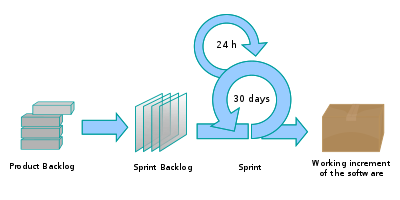
\includegraphics[width=1.0\columnwidth]{images/Scrum_process.png}
\end{center}
\caption{Modello del ciclo di sviluppo software Scrum}
\label{fig:scrum}
\end{figure}


\clearpage


\subsection{Diagramma di Gantt}
Di seguito viene riportato il \gls{diagrammagantt} che indica la suddivisione del lavoro durante tutto il periodo di stage. Il seguente diagramma è stato tracciato con il tutor aziendale Nicola Frongia, e condiviso con il team di sviluppo.\\ 



\begin{figure}
\begin{center}
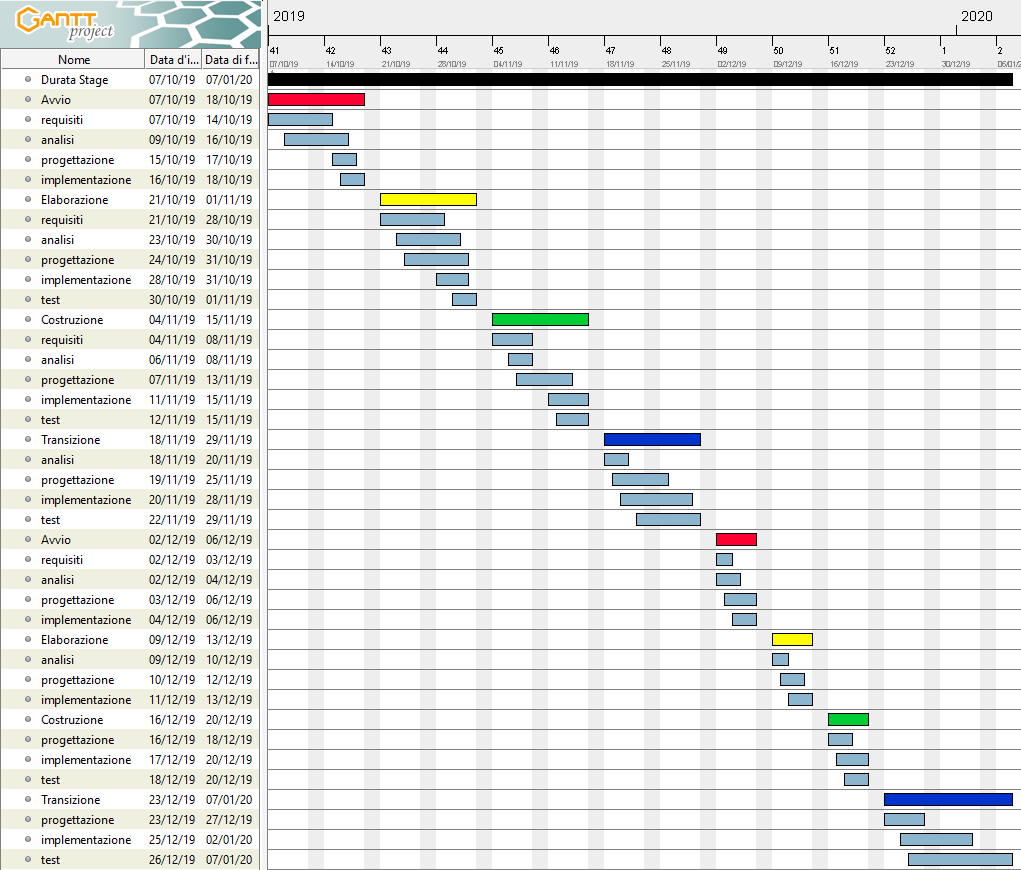
\includegraphics[width=1.0\columnwidth]{images/ganttstoianov.png}
\end{center}
\caption{Diagramma di Gantt per pianificazione dello stage}
\label{fig:gantt}
\end{figure}





\chapter{Strumenti e tecnologie}
\label{chap:strumenti}

In questa sezione vengono introdotti gli strumenti e le tecnologie utilizzate per lo sviluppo della \textit{Web Application}. La scelta di questi si è basata principalmente sulle conoscenze e sull'esperienza del team di sviluppo. 

\section{Spring}

\begin{figure}
\begin{center}

\includegraphics[width=0.5\columnwidth]{images/springlogo.png}
\end{center}
\caption{Logo Spring Framework}
\label{fig:springf}
\end{figure}

Per il \textit{back-end} è stato scelto Spring, che è un \gls{framework} molto utilizzato e supportato per le
moderne applicazioni basate su Java. Il lavoro principale svolto da Spring è la semplificazione dell'unione e dei collegamenti delle parti dell'applicazione, permettendo agli sviluppatori di concentrarsi unicamente sulla logica di business. È basato su
concetti chiave come l’\textit{inversion of control} e la \textit{dependency injection} \cite{spring}.\\

L'\textit{inversion of control} è un pattern per cui un componente di livello applicativo riceve il controllo da un componente appartenente a un libreria. Lo scopo di questo pattern è quello di rendere le parti del sistema software più indipendenti fra loro, ottenendo così la possibilità di effettuare modifiche senza coinvolgere altre parti del sistema \cite{ioc} \cite{baeldung}. \\

La \textit{dependency injection} è il secondo concetto chiave, attraverso questo \gls{designpattern} è possibile implementare l'\textit{inversion of control}. È una tecnica in cui un oggetto acquisisce le dipendenze necessarie in fase di creazione, quando gli viene \textit{iniettato} un oggetto,
il quale viene poi utilizzato come servizio dall’oggetto principale \cite{depinj} \cite{baeldung}.



\subsection{Spring Boot}
\begin{figure}
\begin{center}

\includegraphics[width=0.8\columnwidth]{images/springbootlogo.jpg}
\end{center}
\caption{Logo Spring Boot}
\label{fig:springboot}
\end{figure}

Spring Boot è una soluzione \textit{"convention over configuration"} riduce la complessità di configurazione di nuovi progetti Spring. A questo scopo, Spring Boot definisce una configurazione di base che include le linee guida per l'uso del \gls{framework} e tutte le librerie di terze parti rilevanti, rendendo quindi l'avvio di nuovi progetti il più semplice possibile \cite{springboot}.


\subsection{Spring Data}
\begin{figure}
\begin{center}
\includegraphics[width=0.3\columnwidth]{images/springdata.png}
\end{center}
\caption{Logo Spring Data}
\label{fig:springdata}
\end{figure}
Spring Data ha lo scopo di fornire un modello di programmazione per l'accesso ai dati e per la gestione della persistenza di essi. Definisce un’insieme di \gls{API} per semplificare l'utilizzo di tecnologie che si interfacciano con database relazionali e non. Questo progetto contiene molti sottoprogetti specifici di un determinato database. In particolare nella \textit{Web Application } è stato utilizzato Spring Data JPA che 
fornisce l’accesso a database relazionali e ne permette la gestione tramite oggetti Java.
Il \gls{DBMS} utilizzato è stato Oracle e tramite questo modello è stato possibile mappare le tabelle del database con oggetti \cite{springdata}.

\clearpage

\subsection{Spring Security}

\begin{figure}
\begin{center}

\includegraphics[width=0.45\columnwidth]{images/springsec.jpeg}
\end{center}
\caption{Logo Spring Security}
\label{fig:springsec}
\end{figure}

Spring Security è un \gls{framework} di autenticazione e controllo degli accessi altamente personalizzabile. È lo standard \textit{de facto} per la protezione delle applicazioni basate su Spring. Per garantire l'accesso alla \textit{Web Application} ai soli utenti autorizzati si è utilizzato inoltre il meccanismo di autenticazione \textit{JWT}. Questo meccanismo è diventato uno standard che viene usato per “regolare” le richieste tra  \textit{client} e \textit{server}. Dopo l'esito positivo dell'autenticazione il server genera un \textit{token}, ovvero una stringa \textit{JWT}, contente informazioni specifiche per l'utente, tra cui anche la scadenza del \textit{token}. Ad ogni successiva richiesta da parte del \textit{client} di accedere a determinate risorse del \textit{server}, verrà richiesto il \textit{token} e avverrà il controllo di esso. Di seguito uno schema riassuntivo del meccanismo :

\begin{figure}
\begin{center}
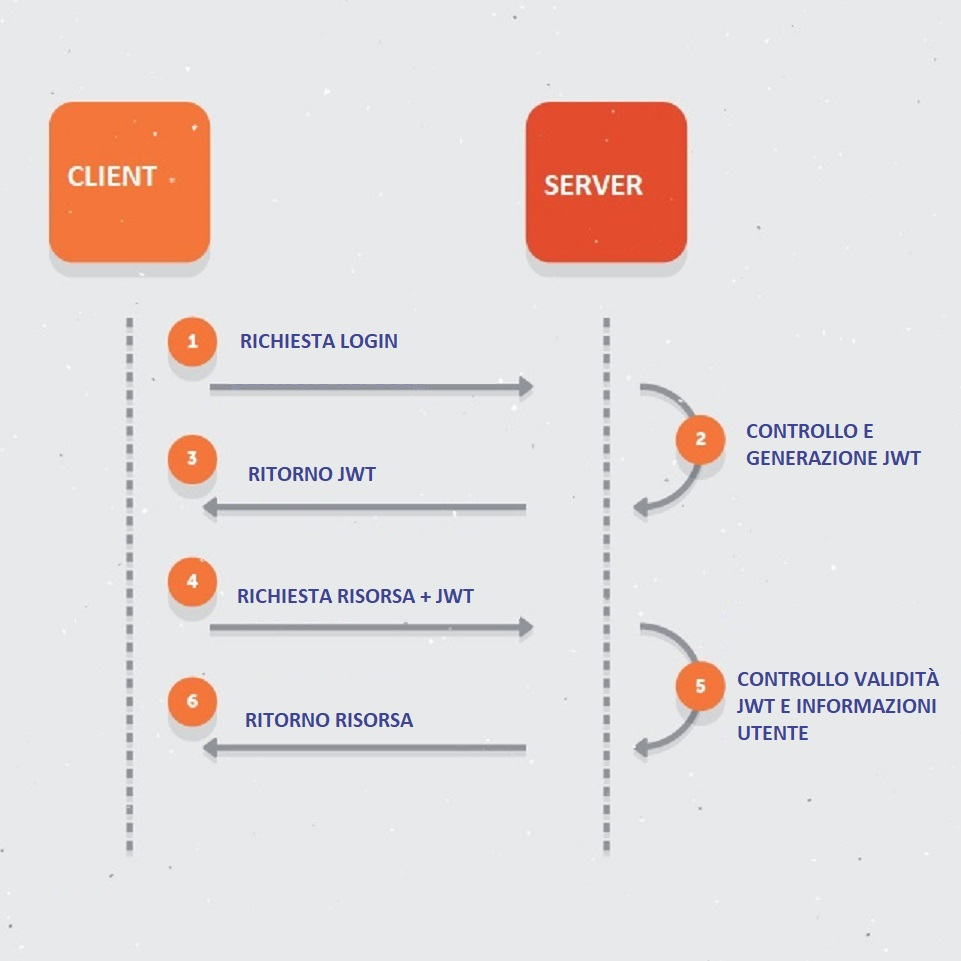
\includegraphics[width=0.6\columnwidth]{images/jwt.jpg}
\end{center}
\caption{Schema riassuntivo meccanismo JWT}
\label{fig:jwt}
\end{figure}



%\foreignlanguage{english}{\Blindtext}

\section{Angular}

\begin{figure}
\begin{center}

\includegraphics[width=0.17\columnwidth]{images/angularlogopng.png}
\end{center}
\caption{Logo Angular}
\label{fig:angular}
\end{figure}

Angular è un \gls{framework} molto utilizzato per lo sviluppo di applicazioni web, in particolar modo della parte riguardante il \textit{front-end}. Sviluppato principalmente da Google, è l'evoluzione del suo predecessore AngulaJS, le due versioni non sono compatibili. Il linguaggio di programmazione usato per la prima versione è JavaScript mentre quello di Angular è TypeScript. Quest'ultimo, è un linguaggio di programmazione sviluppato da Microsoft \cite{angular}.
Nasce dal crescente bisogno di un linguaggio \textit{front-end} per lo sviluppo di applicazioni JavaScript su larga scala e dalla necessità di sicurezza e robustezza.
Il linguaggio estende la sintassi di JavaScript in modo che qualunque programma scritto in JavaScript sia anche in grado di funzionare con TypeScript senza nessuna modifica. È destinato a essere compilato in JavaScript per poter essere interpretato da qualunque web browser \cite{typescript}. I costrutti principali di questo framework sono: \cite{angulararchi}
\begin{itemize}
    \item \textit{Component}: è l’elemento principale di un’applicazione Angular.
    Esso contiene la logica di interazione dati e utente che definisce l’aspetto ed il comportamento della vista. Un \textit{component} quindi è un singolo elemento dell'interfaccia utente, dotato di caratteristiche univoche e che è possibile collegare chiaramente ad altri elementi dell'interfaccia \cite{component}.
    \item \textit{Service}:  è una classe che viene definita per svolgere un compito ben preciso ed effettuare delle operazioni strettamente correlate tenendo in mente il principio di singola responsabilità. Esempi di questi compiti sono: reperimento dei dati dal \textit{server}, gestione degli errori e scambio di dati tra \textit{component} \cite{service}. 
\end{itemize}

\subsection{Bootstrap}

\begin{figure}
\begin{center}

\includegraphics[width=0.11\columnwidth]{images/bootstraplogo.png}
\end{center}
\caption{Logo Bootstrap}
\label{fig:bootstrap}
\end{figure}

Per rendere l'interfaccia grafica più \textit{user-friendly} si è utilizzato Bootstrap, una raccolta di strumenti basati su HTML, CSS e JavaScript che fornisce componenti già formattati e visualmente
piacevoli come bottoni, barre di navigazione, \textit{card} e molti altri.









\chapter{Analisi}
\label{chap:analisi}


\section{Scopo del progetto}
\section{Attori del sistema}

\section{Casi d'uso}
\subsection{Casi d'uso formato breve}
\subsection{Casi d'uso formato dettagliato}
\subsection{Diagramma dei casi d'uso}
\subsection{Definizione requisiti}


\chapter{Progettazione e codifica}
\label{chap:progettazione}

\section{Ambiente di lavoro}
\subsection{Architettura già esistente}

\section{Strumenti di supporto}

\section{Progettazione}

\subsection{Backend}
\subsection{Frontend}
\chapter{Verifica e validazione}
\label{chap:verifica}

\section{Analisi statica}
Per l'analisi statica ed in particolare per alcune metriche come la complessità  ciclomatica, il numero di linee di codice per unità di compilazione e per le \gls{bestpractices} riguaranti la scrittura del codice è stato utilizzato SonarQube. 

\begin{figure}
\begin{center}

\includegraphics[width=0.5\columnwidth]{images/sonarqube-logo.png}
\end{center}
\caption{Logo SonarQube}
\label{fig:sonar}
\end{figure}

SonarQube è una piattaforma \gls{opensource} per la gestione della qualità  del codice. Nello specifico è un’applicazione web che produce \textit{reports} sul codice duplicato, sugli standards di programmazione, i tests di unità , il \textit{code coverage}, la complessità , i \textit{bugs} potenziali, i commenti, la progettazione e l’architettura \cite{sonarqube}.
\section{Analisi dinamica}
Per l'analisi dinamica non è stato utilizzato nessuno strumento in particolare, bensì durante le fasi di collaudo con il committente sono stati effettuati i vari test per verificare la correttezza del programma e dell'analisi effettuata. La fase finale di collaudo, effettuata le ultime due settimane prima del rilascio del progetto, è stata fondamentale per la correzione degli ultimi errori rimasti.

\chapter{Conclusioni e sviluppi futuri}
\label{chap:conclusioni}

\section{Valutazione personale}
La \textit{Web Application} sviluppata è attualmente utilizzata in ambiente di produzione del committente. Posso ritenere dunque, l'esperienza di grande aiuto a livello professionale e personale, poichè mi ha permesso di lavorare ad un progetto importante dove ho potuto mettere in campo tutte le competenze acquisite durante il corso di studio e durante una formazione specifica aziendale. Inoltre, quest'esperienza ha arricchito notevolmente il mio bagaglio di conoscenze e l'aver lavorato in un team di sviluppo già competente ed organizzato ha alzato il mio livello di capacità di collaborazione e di suddivisione dei compiti. Non posso che valutare l'intera esperienza molto positivamente e ringraziare l'azienda presso la quale sono stato assunto dell'opportunità che mi è stata data.



\section{Sviluppi futuri}

Per la \textit{Web application} sono stati già individuati dei possibili sviluppi futuri che il committente potrebbe richiedere:
\begin{itemize}
    \item Installazione su entrambi i nodi dell'architettura, con la gestione della concorrenza dei flussi da parte dell'applicazione.
    \item Integrazione con altri sistemi presenti all'interno della struttura del committente.
    \item Possibilità di copiare flussi esistenti.
    \item Integrazione con ulteriori \gls{API} del sistema.
    \item Monitoraggio del ciclo di vita di un flusso.
\end{itemize}


\appendix
% INCLUSIONE APPENDICI - - PERSONALIZZARE - TENERE COERENTE CON LISTA IN ALTO
\chapter{Appendice}
\label{app:a}
% DA RIMUOVERE - LOREM IPSUM PER DIMOSTRAZIONE
%\foreignlanguage{english}{\Blindtext}


%%%%%%%%%%%%%%%%%%%%%%%%%%%%%%%%%%%%%%%%%%%%%%%%%%%%%%%%%%%%%%%
% %GLOSSARIO
\phantomsection
%\addcontentsline{toc}{chapter}{Glossario}
% \hypertarget{glossario}{}
\printglossary
\clearpage





%%%%%%%%%%%%%%%%%%%%%%%%%%%%%%%%%%%%%%%%%%%%%%%%%%%%%%%%%%%%%%%

% BIBLIOGRAFIA
\phantomsection
\addcontentsline{toc}{chapter}{\refname}
\nocite{*}
\printbibliography

\end{document}
